%{{第七十三回}}{第七十三回}}
\chapter{痴丫头误拾绣春囊\\懦小姐不问累金凤}
{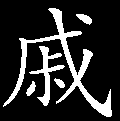
\includegraphics[width=3mm]{../Images/00005}\kaishu 贾母一席话,隐隐照起全文,便可一直叙去,接笔却置贼不论,转出赌钱,接笔又置赌钱不论,转出奸证,接笔又置奸证不论,转出讨情,一波未平,一波又起,势如怒蛇出穴,蜿蜒不就捕。}

话说那赵姨娘和贾政说话,忽听外面一声响,不知何物。忙问时,\elegantpar{原来是外间窗屉不曾扣好,塌了屈戌了吊下来}{并非全新}。赵姨娘骂了丫头几句,自己带领丫鬟上好,方进来打发贾政安歇。不在话下。

却说怡红院中宝玉正才睡下,丫鬟们正欲各散安歇,忽听有人击院门。老婆子开了门,见是赵姨娘房内的丫鬟名唤小鹊的。问他什么事,小鹊不答,直往房内来找宝玉。{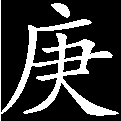
\includegraphics[width=3mm]{../Images/00004}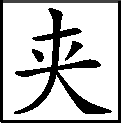
\includegraphics[width=3mm]{../Images/00012}\footnotesize \kaishu 奇,从未见此婢也。}只见宝玉才睡下,晴雯等犹在床边坐着,大家顽笑,见他来了,都问:``什么事,这时候又跑了来作什么?''{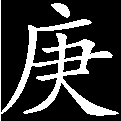
\includegraphics[width=3mm]{../Images/00004}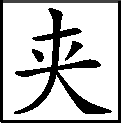
\includegraphics[width=3mm]{../Images/00012}\footnotesize \kaishu 又是补出前文矣,非只{(张)}{[}此{]}一回也。}小鹊笑向宝玉道:``我来告诉你一个信儿。方才我们奶奶这般如此在老爷前说了。你仔细明儿老爷问你话。''说着回身就去了。袭人命留他吃茶,因怕关门,遂一直去了。

这里宝玉听了,便如孙大圣听见了紧箍咒一般,登时四肢五内一齐皆不自在起来。想来想去,别无他法,且理熟了书预备明儿盘考。口内不舛错,便有他事,也可搪塞一半。想罢,忙披衣起来要读书。心中又自后悔,这些日子只说不提了,偏又丢生,早知该天天好歹温习些的。如今打算打算,肚子内现可背诵的,不过``学''、``庸''、二``论'',是带注背得出的。至上本《孟子》,就有一半是夹生的,若凭空提一句,断不能接背的,至``下孟'',就有一大半忘了。算起``五经''来,因近来作诗,常把《诗经》读些,虽不甚精阐,还可塞责。{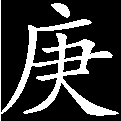
\includegraphics[width=3mm]{../Images/00004}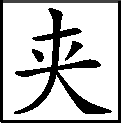
\includegraphics[width=3mm]{../Images/00012}\footnotesize \kaishu 妙!宝玉读书原系从{(问)}{[}闺{]}中{(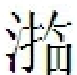
\includegraphics[width=4mm]{../images/00030})}{[}滥{]}}\href{../Text/part0077_split_000.html\#lnkback_1_a}{\textsuperscript{①}}{而有。}别的虽不记得,素日贾政也幸未吩咐过读的,纵不知,也还不妨。至于古文,这是那几年所读过的几篇,连《左传》、《国策》、《公羊》、《谷粱》、汉唐等文,不过几十篇,这几年竟未曾温得半篇片语,虽闲时也曾遍阅,不过一时之兴,随看随忘,未下苦工夫,如何记得。这是断难塞责的。更有时文八股一道,因平素深恶此道,原非圣贤之制撰,焉能阐发圣贤之微奥,\elegantpar{不过作后人饵名钓禄之阶}{经济之书,时尚之学。}。虽贾政当日起身时选了百十篇命他读的,不过偶因见其中或一二股内,或承起之中,有作的或精致,或流荡,或游戏,或悲感,稍能动性者,偶一读之,不过供一时之兴趣,究竟何曾成篇潜心玩索。{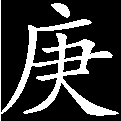
\includegraphics[width=3mm]{../Images/00004}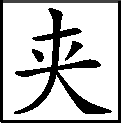
\includegraphics[width=3mm]{../Images/00012}\footnotesize \kaishu 妙!写宝玉读书非为功名也。}如今若温习这个,又恐明日盘诘那个,若温习那个,又恐盘驳这个。况一夜之功,亦不能全然温习,因此越添了焦燥。自己读书不致紧要,却带累着一房丫鬟们皆不能睡。袭人、麝月、晴雯等几个大的自不用说,在旁剪烛斟茶,那些小的,都困眼朦胧,前仰后合起来。晴雯因骂道:``什么蹄子们,一个个黑日白夜挺尸挺不够,偶然一次睡迟了些,就装出这腔调来了。再这样,我拿针戳给你们两下子!''

话犹未了,只听外间``咕咚''一声,急忙看时,原来是一个小丫头子坐着打盹,一头撞到壁上了,从梦中惊醒,恰正是晴雯说这话之时,他怔怔的只当是晴雯打了他一下,遂哭央说:``\elegantpar{好姐姐,我再不敢了。}{好姐姐,我再不敢了。}''众人都发起笑来。

宝玉忙劝道:``饶他去罢,原该叫他们都睡去才是。你们也该替换着睡去。''袭人忙道:``小祖宗,你只顾你的罢。通共这一夜的工夫,你把心暂且用在这几本书上,等过了这一关,由你再张罗别的去,也不算误了什么。''宝玉听他说的恳切,只得又读。读了没有几句,麝月又斟了一杯茶来润舌,宝玉接茶吃了。因见麝月只穿着短袄,解了裙子,宝玉道:``夜静了,冷,到底穿一件大衣裳才是。''麝月笑指着书道:``你暂且把我们忘了,心且略对着他些罢。''{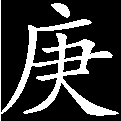
\includegraphics[width=3mm]{../Images/00004}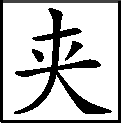
\includegraphics[width=3mm]{../Images/00012}\footnotesize \kaishu 此处岂是读书之处,又岂是伴读之人?古今天下误尽多少纨绔!何况又是此等时之怡红院,此等之鬟婢,又是此等一个宝玉哉!}

话犹未了,只听金星玻璃从后房门跑进来,口内喊说:``不好了,一个人从墙上跳下来了!''众人听说,忙问在那里,即喝起人来,各处寻找。晴雯因见宝玉读书苦恼,劳费一夜神思,明日也未必妥当,心下正要替宝玉想出一个主意来脱此难,正好忽然逢此一惊,即便生计,向宝玉道:``趁这个机会快装病,只说唬着了。''此话正中宝玉心怀,因而遂传起上夜人等来,打着灯笼,各处搜寻,并无踪迹,都说:``小姑娘们想是睡花了眼出去,风摇的树枝儿,错认作人了。''晴雯便道:``别放诌屁!你们查的不严,怕得不是,还拿这话来支吾。才刚并不是一个人见的,宝玉和我们出去有事,大家亲见的。如今宝玉唬的颜色都变了,满身发热,我如今还要上房里取安魂丸药去。太太问起来,是要回明白的,难道依你说就罢了不成。''

众人听了,吓的不敢则声,只得又各处去找。晴雯和玻璃二人果出去要药,故意闹的众人皆知宝玉吓着了。王夫人听了,忙命人来看视给药,又吩咐各上夜人仔细搜查,又一面叫查二门外邻园墙上夜的小厮们。于是园内灯笼火把,直闹了一夜。至五更天,就传管家男女,命仔细查一查,拷问内外上夜男女等人。

贾母闻知宝玉被吓,细问原由。不敢再隐,只得回明。贾母道:``我必料到有此事。如今各处上夜都不小心,还是小事,只怕他们就是贼也未可知。''当下邢夫人并尤氏等都过来请安,凤姐及李纨姊妹等皆陪侍,听贾母如此说,都默无所答。独探春出位笑道:``近因凤姐姐身子不好,几日园内的人比先放肆了许多。先前不过是大家偷着一时半刻,或夜里坐更时,三四个人聚在一处,或掷骰或斗牌,小小的顽意,不过为熬困。近来渐次放诞,竟开了赌局,甚至有头家局主,或三十吊五十吊三百吊的大输赢。半月前竟有争斗相打之事。''贾母听了,忙说:``你既知道,为何不早回我们来?''探春道:``我因想着太太事多,且连日不自在,所以没回。只告诉了大嫂子和管事的人们,戒饬过几次,近日好些。''贾母忙道:``你姑娘家,如何知道这里头的利害。\elegantpar{你自为耍钱常事,不过怕起争端。殊不知夜间既耍钱,就保不住不吃酒,既吃酒,就免不得门户任意开锁。或买东西,寻张觅李,其中夜静人稀,趁便藏贼引盗,何等事作不出来。}{是也}况且园内的姊妹们起居所伴者皆系丫头媳妇们,贤愚混杂,贼盗事小,再有别事,倘略沾带些,关系不小。这事岂可轻恕。''探春听说,便默然归坐。凤姐虽未大愈,精神因此比常稍减,{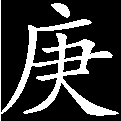
\includegraphics[width=3mm]{../Images/00004}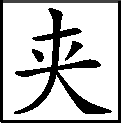
\includegraphics[width=3mm]{../Images/00012}\footnotesize \kaishu 看他渐次写来,从不作一笔安逸之笔,}\href{../Text/part0077_split_000.html\#lnkback_2_a}{\textsuperscript{②}}{况阿凤之文哉。}今见贾母如此说,便忙道:``偏生我又病了。''遂回头命人速传林之孝家的等总理家事四个媳妇到来,当着贾母申饬了一顿。贾母命即刻查了头家赌家来,有人出首者赏,隐情不告者罚。

林之孝家的等见贾母动怒,谁敢徇私,忙至园内传齐人,一一盘查。虽不免大家赖一回,终不免水落石出。查得大头家三人,小头家八人,聚赌者通共二十多人,都带来见贾母,跪在院内磕响头求饶。贾母先问大头家名姓和钱之多少。原来这三个大头家,一个就是林之孝家的两姨亲家,一个就是园内厨房内柳家媳妇之妹,一个就是迎春之乳母。这是三个为首的,馀者不能多记。

贾母便命将骰子牌一并烧毁,所有的钱入官分散与众人,将为首者每人四十大板,撵出,总不许再入;从者每人二十大板,革去三月月钱,拨入圊厕行内。又将林之孝家的申饬了一番。林之孝家的见他的亲戚又与他打嘴,自己也觉没趣。

迎春在坐,也觉没意思。黛玉、宝钗、探春等见迎春的乳母如此,也是物伤其类的意思,遂都起身笑向贾母讨情说:``这个妈妈素日原不顽的,不知怎么也偶然高兴。求看二姐姐面上,饶他这次罢。''贾母道:``你们不知。大约这些奶子们,一个个仗着奶过哥儿姐儿,原比别人有些体面,他们就生事,比别人更可恶,专管调唆主子护短偏向。我都是经过的。况且要拿一个作法,恰好果然就遇见了一个。你们别管,我自有道理。''宝钗等听说,只得罢了。

一时贾母歇晌,大家散出,都知贾母今日生气,皆不敢各散回家,只得在此暂候。尤氏便往凤姐处来闲话了一回,因他也不自在,只得往园内寻众姑嫂闲谈。邢夫人在王夫人处坐了一回,也就往园内散散心来。刚至园门前,只见贾母房内的小丫头子名唤傻大姐的笑嘻嘻走来,手内拿着个花红柳绿的东西,低头一壁瞧着,一壁只管走,不防迎头撞见邢夫人,抬头看见,方才站住。邢夫人因说:``这痴丫头,又得了个什么狗不识儿这么欢喜?拿来我瞧瞧。''

原来这傻大姐年方十四五岁,是新挑上来的与贾母这边提水桶扫院子专作粗活的一个丫头。只因他生得体肥面阔,两只大脚,作粗活简捷爽利,且心性愚顽,一无知识,行事出言,常在规矩之外。贾母因喜欢他爽利便捷,又喜他出言可以发笑,便起名为``呆大姐'',常闷来便引他取笑一回,毫无避忌,因此又叫他作``痴丫头''。他纵有失礼之处,见贾母喜欢他,众人也就不去苛责。

这丫头也得了这个力,若贾母不唤他时,便入园内来顽耍。今日正在园内掏促织,忽在山石背后得了一个五彩绣香囊,其华丽精致,固是可爱,但上面绣的并非花鸟等物,一面却是\elegantpar{两个人赤条条的盘踞相抱}{韦小宝心头爱},一面是几个字。这痴丫头原不认得是春意,便心下盘算:``敢是两个妖精打架?不然必是两口子相打。''左右猜解不来,正要拿去与贾母看,{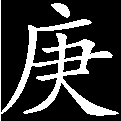
\includegraphics[width=3mm]{../Images/00004}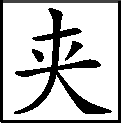
\includegraphics[width=3mm]{../Images/00012}\footnotesize \kaishu 险极,妙极!荣府堂堂诗礼之家,且大观官园又何等严肃清幽之地,金闺玉阁尚有此等秽物,天下浅闺薄幕之家宁不慎乎!虽然,但此等偏出大官世族之中者,盖因其房室香宵、鬟婢混杂,焉保其个个守礼持节哉?此正为大官世族而告诫。其浅闺薄幕之处,毋如主婢日夕耳鬓交磨,一止一动悉在耳目之中,又何必谆谆再四焉!}\href{../Text/part0077_split_000.html\#lnkback_3_a}{\textsuperscript{③}}是以笑嘻嘻的一壁看,一壁走,忽见了邢夫人如此说,便笑道:``太太真个说的巧,真个是狗不识呢。{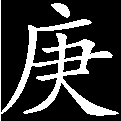
\includegraphics[width=3mm]{../Images/00004}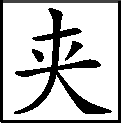
\includegraphics[width=3mm]{../Images/00012}\footnotesize \kaishu 妙!寓言也,大凡知此交媾之情者,真狗畜之识耳,非肆言恶詈凡识此事者即狗矣。然则云与贾母看,则先骂贾母矣。此处邢夫人亦看,然则又骂邢夫人乎?故作者又难。}太太请瞧一瞧。''说着,便送过去。

邢夫人接来一看,吓得连忙死紧攥住,{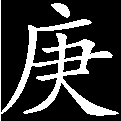
\includegraphics[width=3mm]{../Images/00004}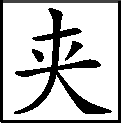
\includegraphics[width=3mm]{../Images/00012}\footnotesize \kaishu 妙!这一``吓''字方是写世家夫人之笔。虽前文明书邢夫人之为人稍劣,然{(不)}{[}亦{]}在情理之中,若不用慎重之笔,则邢夫人直系一小家卑污极轻贱之人矣,岂得与荣府联房哉?所谓此书针线慎密处,全在无意中一字一句之间耳,看者细心方得。}忙问:``你是那里得的?''傻大姐道:``我掏促织儿在山石上拣的。''邢夫人道:``快休告诉一人。这不是好东西,连你也要打死。皆因你素日是傻子,以后再别提起了。''这傻大姐听了,反吓的黄了脸,说:``再不敢了。''磕了个头,呆呆而去。邢夫人回头看时,都是些女孩儿,不便递与,自己便塞在袖内,心内十分罕异,揣摩此物从何而至,且不形于声色,且来至迎春室中。

迎春正因他乳母获罪,自觉无趣,心中不自在,忽报母亲来了,遂接入内室。奉茶毕,邢夫人因说道:``你这么大了,你那奶妈子行此事,你也不说说他。如今别人都好好的,偏咱们的人做出这事来,什么意思。''{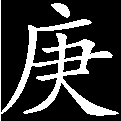
\includegraphics[width=3mm]{../Images/00004}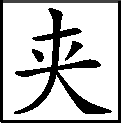
\includegraphics[width=3mm]{../Images/00012}\footnotesize \kaishu ``咱们''二字便见自怀异心,从上文生离异发沥而来,谨密之至。更有人{[}甚{]}于此者,君未知也,一笑。}迎春低着头弄衣带,半晌答道:``我说他两次,他不听也无法。况且他是妈妈,只有他说我的,没有我说他的。''{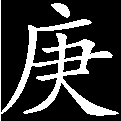
\includegraphics[width=3mm]{../Images/00004}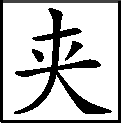
\includegraphics[width=3mm]{../Images/00012}\footnotesize \kaishu 妙极!直画出一个懦弱小姐来。}邢夫人道:``胡说!你不好了他原该说,如今他犯了法,你就该拿出小姐的身分来。他敢不从,你就回我去才是。如今直等外人共知,是什么意思。{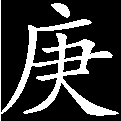
\includegraphics[width=3mm]{../Images/00004}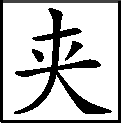
\includegraphics[width=3mm]{../Images/00012}\footnotesize \kaishu 我敬问:``外人''为谁?}再者,只他去放头儿,还恐怕他巧言花语的和你借贷些簪环衣履作本钱,你这心活面软,未必不周接他些。若被他骗去,我是一个钱没有的,看你明日怎么过节。''迎春不语,只低头弄衣带。

邢夫人见他这般,因冷笑道:``总是你那好哥哥好嫂子,一对儿赫赫扬扬,琏二爷凤奶奶,两口子遮天盖日,百事周到,竟通共这一个妹子,全不在意。{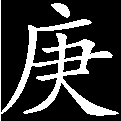
\includegraphics[width=3mm]{../Images/00004}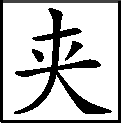
\includegraphics[width=3mm]{../Images/00012}\footnotesize \kaishu 加{(在)}{[}罪{]}于琏凤,的是父母常情,极是。何必又如此说来,便见又有私意。}但凡是我身上掉下来的,又有一话说------只好凭他们罢了。{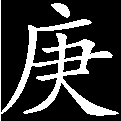
\includegraphics[width=3mm]{../Images/00004}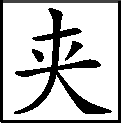
\includegraphics[width=3mm]{../Images/00012}\footnotesize \kaishu 如何?此皆妇女私假之意,大不可者。}况且你又不是我养的,{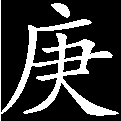
\includegraphics[width=3mm]{../Images/00004}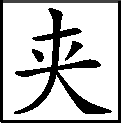
\includegraphics[width=3mm]{../Images/00012}\footnotesize \kaishu 更不好。}你虽然不是同他一娘所生,到底是同出一父,也该彼此瞻顾些,也免别人笑话。{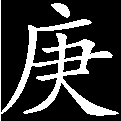
\includegraphics[width=3mm]{../Images/00004}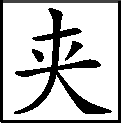
\includegraphics[width=3mm]{../Images/00012}\footnotesize \kaishu 又问:``别人''为谁?又问:彼二人虽不同母,终是同父。彼二人既同父,其父又系君之何人?吁!妇人私心,今古有之。}我想天下的事也难较定,你是大老爷跟前人养的,这里探丫头也是二老爷跟前人养的,出身一样。如今你娘死了,从前看来,你两个的娘,只有你娘比如今赵姨娘强十倍的,你该比探丫头强才是。怎么反不及他一半?谁知竟不然,这可不是异事!\href{../Text/part0077_split_000.html\#lnkback_4_a}{\textsuperscript{④}}倒是我一生无儿无女的,一生干净,也不能惹人笑话议论为高。''{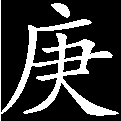
\includegraphics[width=3mm]{../Images/00004}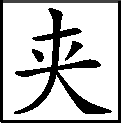
\includegraphics[width=3mm]{../Images/00012}\footnotesize \kaishu 最可恨妇人无子者引此话{(是)}{[}饰{]}说。}旁边伺候的媳妇们便趁机道:``我们的姑娘老实仁德,那里像他们三姑娘伶牙俐齿,会要姊妹们的强。他们明知姐姐这样,他竟不顾恤一点儿。''{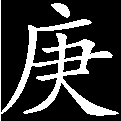
\includegraphics[width=3mm]{../Images/00004}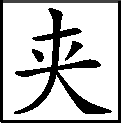
\includegraphics[width=3mm]{../Images/00012}\footnotesize \kaishu 杀杀杀!此辈专生离异。余因实受其蛊,今读此文,直欲拔剑劈纸。又不知作者多少眼泪洒出此回也。又问不知如何``顾恤''些,又不知有何可``顾恤''之处,直令人不解。愚奴贱婢之言,酷肖之至!}邢夫人道:``连他哥哥嫂子还如是,别人又作什么呢。''一言未了,人回:``琏二奶奶来了。''邢夫人听了,冷笑两声,命人出去说:``请他自去养病,我这里不用他伺候。''接着又有探事的小丫头来报说:``老太太醒了。''邢夫人方起身前边来。迎春送至院外方回。

绣橘因说道:``如何,前儿我回姑娘,那一个攒珠累丝金凤竟不知那里去了。回了姑娘,姑娘竟不问一声儿。我说必是老奶奶拿去典了银子放头儿的,姑娘不信,只说司棋收着呢。问司棋,司棋虽病着,心里却明白。我去问他,他说没有收起来,还在书架上匣内暂放着,预备八月十五日恐怕要戴呢。姑娘就该问老奶奶一声,只是脸软怕人恼。如今竟怕无着,明儿要都戴时,独咱们不戴,是何意思呢。''{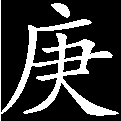
\includegraphics[width=3mm]{../Images/00004}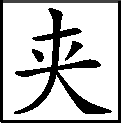
\includegraphics[width=3mm]{../Images/00012}\footnotesize \kaishu 这个``咱们''使得恰,是女儿喁喁私语,非前文之一例可比者。写得出,批得出。}

迎春道:``何用问,自然是他拿去暂时借一肩了。我只说他悄悄的拿了去,不过一日半晌,仍旧悄悄的送了来,谁知他就忘了。今日偏又闹出来,问他想也无益。''绣橘道:``何曾是忘记!他是试准了姑娘的性格,所以才这样。如今我有个主意:我竟走到二奶奶房里将此事回了他,或他着人去要,或他省事拿几吊钱来替他赔补。如何?''{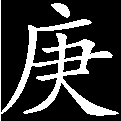
\includegraphics[width=3mm]{../Images/00004}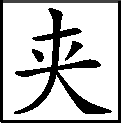
\includegraphics[width=3mm]{../Images/00012}\footnotesize \kaishu 写女儿各有机变,个个不同。}迎春忙道:``罢,罢,罢,省些事罢。宁可没有了,又何必生事。''{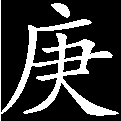
\includegraphics[width=3mm]{../Images/00004}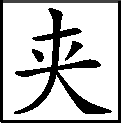
\includegraphics[width=3mm]{../Images/00012}\footnotesize \kaishu 总是懦语。}绣橘道:``姑娘怎么这样软弱。都要省起事来,将来连姑娘还骗了去呢,我竟去的是。''说着便走。迎春便不言语,只好由他。

谁知迎春乳母子媳王住儿媳妇正因他婆婆得了罪,来求迎春去讨情,听他们正说金凤一事,且不进去。也因素日迎春懦弱,他们都不放在心上。如今见绣橘立意去回凤姐,估着这事脱不去的,且又有求迎春之事,只得进来,陪笑先向绣橘说:``姑娘,你别去生事。姑娘的金丝凤,原是我们老奶奶老糊涂了,输了几个钱,没的捞梢,所以暂借了去。\elegantpar{原说一日半晌就赎的,因总未捞过本儿来,就迟住了}{赌场上有什么尽头}。可巧今儿又不知是谁走了风声,弄出事来。虽然这样,到底主子的东西,我们不敢迟误下,终久是要赎的。如今还要求姑娘看从小儿吃奶的情常,往老太太那边去讨个情面,救出他老人家来才好。''迎春先便说道:``好嫂子,你趁早儿打了这妄想,要等我去说情儿,等到明年也不中用的。方才连宝姐姐林妹妹大伙儿说情,老太太还不依,何况是我一个人。我自己愧还愧不来,反去讨臊去。''绣橘便说:``赎金凤是一件事,说情是一件事,别绞在一处说。难道姑娘不去说情,你就不赎了不成?嫂子且取了金凤来再说。''

王住儿家的听见迎春如此拒绝他,绣橘的话又锋利无可回答,一时脸上过不去,也明欺迎春素日好性儿,乃向绣橘发话道:``姑娘,你别太仗势了。你满家子算一算,谁的妈妈奶子不仗着主子哥儿多得些益,偏咱们就这样丁是丁卯是卯的,只许你们偷偷摸摸的哄骗了去。自从邢姑娘来了,太太吩咐一个月俭省出一两银子来与舅太太去,这里饶添了邢姑娘的使费,反少了一两银子。常时短了这个,少了那个,那不是我们供给?谁又要去?不过大家将就些罢了。算到今日,少说些也有三十两了。我们这一向的钱,岂不白填了限呢。''绣橘不待说完,便啐了一口,道:``作什么的白填了三十两,我且和你算算账,姑娘要了些什么东西?''迎春听见这媳妇发邢夫人之私意,{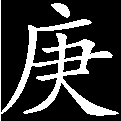
\includegraphics[width=3mm]{../Images/00004}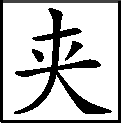
\includegraphics[width=3mm]{../Images/00012}\footnotesize \kaishu 大书此句,诛心之笔。}忙止道:``罢,罢,罢。你不能拿了金凤来,不必牵三扯四乱嚷。我也不要那凤了。便是太太们问时,我只说丢了,也妨碍不着你什么的,出去歇息歇息倒好。''一面叫绣橘倒茶来。

绣橘又气又急,因说道:``姑娘虽不怕,我们是作什么的,把姑娘的东西丢了。他倒赖说姑娘使了他们的钱,这如今竟要准折起来。倘或太太问姑娘为什么使了这些钱,敢是我们就中取势了?这还了得!''一行说,一行就哭了。司棋听不过,只得勉强过来,帮着绣橘问着那媳妇。迎春劝止不住,自拿了一本《太上感应篇》来看。{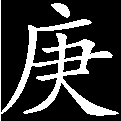
\includegraphics[width=3mm]{../Images/00004}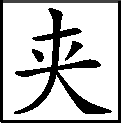
\includegraphics[width=3mm]{../Images/00012}\footnotesize \kaishu 神妙之至!从纸上跳出一位懦弱小姐,且书又有奇文,妙!}

三人正没开交,可巧宝钗、黛玉、宝琴、探春等因恐迎春今日不自在,都约来安慰他。走至院中,听得两三个人较口。探春从纱窗内一看,只见迎春倚在床上看书,若有不闻之状。{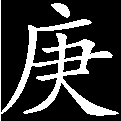
\includegraphics[width=3mm]{../Images/00004}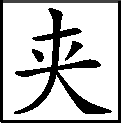
\includegraphics[width=3mm]{../Images/00012}\footnotesize \kaishu 看他写迎春,虽稍劣,然亦大家千金之格也。}探春也笑了。小丫鬟们忙打起帘子,报道:``姑娘们来了。''迎春方放下书起身。那媳妇见有人来,且又有探春在内,不劝而自止了,遂趁便要去。

探春坐下,便问:``才刚谁在这里说话?倒像拌嘴似的。''{\includegraphics[width=3mm]{../Images/00004}\includegraphics[width=3mm]{../Images/00012}\footnotesize \kaishu 瞧他写探春气宇。}迎春笑道:``没有说什么,左不过是他们小题大作罢了。何必问他。''探春笑道:``我才听见什么`金凤',又是什么`没有钱只和我们奴才要',谁和奴才要钱了?难道姐姐和奴才要钱了不成?难道姐姐不是和我们一样有月钱的,一样有用度不成?''司棋绣橘道:``姑娘说的是了。姑娘们都是一样的,那一位姑娘的钱不是由着奶奶妈妈们使,连我们也不知道怎么是算账,不过要东西只说得一声儿。如今他偏要说姑娘使过了头儿,他赔出许多来了。究竟姑娘何曾和他要什么了。''

探春笑道:``姐姐既没有和他要,必定是我们或者和他们要了不成!你叫他进来,我倒要问问他。''迎春笑道:``这话又可笑。你们又无沾碍,何得带累于他。''探春笑道:``这倒不然。和\href{../Text/part0077_split_000.html\#lnkback_5_a}{\textsuperscript{⑤}}姐姐听见也即同怨姐姐是一理。咱们是主子,自然不理论那些钱财小事,只知想起什么要什么,也是有的事。但不知金累丝凤因何又夹在里头?''那王住儿媳妇生恐绣橘等告出他来,遂忙进来用话掩饰。探春深知其意,因笑道:``你们所以糊涂。如今你奶奶已得了不是,趁此求求二奶奶,把方才的钱尚未散人的拿出些来赎取了就完了。比不得没闹出来,大家都藏着留脸面,如今既是没了脸,趁此时纵有十个罪,也只一人受罚,没有砍两颗头的理。你依我,竟是和二奶奶说说。在这里大声小气,如何使得。''

这媳妇被探春说出真病,也无可赖了,只不敢往凤姐处自首。探春笑道:``我不听见便罢,既听见,少不得替你们分解分解。''谁知探春早使个眼色与待书出去了。

这里正说话,忽见平儿进来。宝琴拍手笑说道:``三姐姐敢是有驱神召将的符术?''黛玉笑道:``这倒不是道家玄术,倒是用兵最精的,所谓`守如处女,脱如狡兔',出其不备之妙策也。''二人取笑。宝钗便使眼色与二人,令其不可,遂以别话岔开。探春见平儿来了,遂问:``你奶奶可好些了?真是病糊涂了,事事都不在心上,叫我们受这样的委曲。''平儿忙道:``姑娘怎么委曲?谁敢给姑娘气受,姑娘快吩咐我。''

当时住儿媳妇儿方慌了手脚,遂上来赶着平儿叫:``姑娘坐下,让我说原故请听。''平儿正色道:``姑娘这里说话,也有你我混插口的礼!你但凡知礼,只该在外头伺候。不叫你,进不来的地方,几时有外头的媳妇子们无故到姑娘们房里来的?''绣橘道:``你不知我们这屋里是没礼的,谁爱来就来。''平儿道:``都是你们的不是。姑娘好性儿,你们就该打出去,然后再回太太去才是。''王住儿媳妇见平儿出了言,红了脸方退出去。

探春接着道:``我且告诉你,若是别人得罪了我,倒还罢了。如今那住儿媳妇和他婆婆仗着是妈妈,又瞅着二姐姐好性儿,如此这般私自拿了首饰去赌钱,而且还捏造假账妙算,威逼着还要去讨情,和这两个丫头在卧房里大嚷大叫,二姐姐竟不能辖治,所以我看不过,才请你来问一声:还是他原是天外的人,不知道理?还是谁主使他如此,先把二姐姐制伏,然后就要治我和四姑娘了?''平儿忙陪笑道:``姑娘怎么今日说这话出来?我们奶奶如何当得起!''

探春冷笑道:``俗语说的,`物伤其类',`齿竭唇亡',我自然有些惊心。''平儿道:``若论此事,还不是大事,极好处置。但他现是姑娘的奶嫂,据姑娘怎么样为是?''当下迎春只和宝钗阅《感应篇》故事,究竟连探春之语亦不曾闻得,忽见平儿如此说,乃笑道:``问我,我也没什么法子。他们的不是,自作自受,我也不能讨情,我也不去苛责就是了。至于私自拿去的东西,送来我收下,不送来我也不要了。太太们要问,我可以隐瞒遮饰过去,是他的造化,若瞒不住,我也没法,没有个为他们反欺枉太太们的理,少不得直说。你们若说我好性儿,没个决断,竟有好主意可以八面周全,不使太太们生气,任凭你们处治,我总不知道。''

众人听了,都好笑起来。黛玉笑道:``真是`虎狼屯于阶陛,尚谈因果'。若使二姐姐是个男人,这一家上下若许人,又如何裁治他们。''迎春笑道:``正是。多少男人尚如此,何况我哉?''一语未了,只见又有一人进来。正不知道是那个,且听下回分解。

{\includegraphics[width=3mm]{../Images/00005}\kaishu 总评:一篇奸盗淫邪文字,反以四子书五经、《公羊》、《谷梁》、秦汉诸作起,以《太上感应篇》结,彼何心哉!他深见``书中自有黄金屋''、``书中有女美如玉''等语误尽天下苍生,而大奸大盗皆从此出。故特作此一起结,为五阴浊世顶门一声棒喝也。眼空似箕,笔大如椽,何得以寻行数墨绳之。}

{\kaishu 探春处处出头,人谓其能,吾谓其苦;迎春处处藏舌,人谓其怯,吾谓其超。探春运符咒,固足役鬼驱神;迎春说因果,更可降狼伏虎。}

% {\href{../Text/part0077_split_000.html\#navto_1_a}{①}``问中\includegraphics{../images/00030}'',意义不明。俞平伯先生谓``问,疑闺字。''而``\includegraphics[width=3mm]{../images/00030}''则字书不收,已无法判断因何而致讹了。今姑以形讹校为``滥''字。按``滥''古有``沉浸''之义(现在某些地方方言,例如闽南、潮州还有此用法),``闺中滥'',即``沉浸于闺阁中''也。此意符合批者在第二十二回评价宝玉所作长批``源泉自甘''条,可参看。}

% {\href{../Text/part0077_split_000.html\#navto_2_a}{②}原误作``不作一年易安之笔'',参第七回批``不作一笔逸安之板矣''、第十三回批``全无安逸之笔''、第十七回批``誓不作一笔逸安苟且之笔''而校改。}

% {\href{../Text/part0077_split_000.html\#navto_3_a}{③}此批原文作``险极妙极荣富堂堂诗礼之家且大观官园又何等严肃清幽之地金闺玉阁尚有此等秽妙天下浅闲浦募之家宁不慎乎虽然但此等偏出大官世族之中者盖因其房宝香宵鬟婢混杀鸟保其个个守礼特节哉此正为大官世族而告戒其浅闲浦募之处毋如主婢日夕耳鬓交磨一止一动悉在耳目之中又何必谆谆再四焉'',错字甚多,经过俞平伯、朱一玄、陈庆浩、郑红枫诸先生辑评本的接力校订,大部分问题已经解决。惟``房室香宵''尚费解,联系上下文意,如指大官世族之家房舍多、人口杂,管理不到位,似可校为``房室幽深'',按``幽''``香''形近,``深''则与``浅闺''之``浅''相对。一说``房室香宵''指房事,虽与上下文意不甚吻合,亦勉强可通。}

% {\href{../Text/part0077_split_000.html\#navto_4_a}{④}``怎么反不及他一半''、``谁知竟不然,这可不是异事'',此两句意思重复,而且叠加在一起,造成语气不连贯。这也许是在传抄过程把母本中的初稿和改稿一并抄录的结果。除甲辰本删去后句外,馀本均同底本。}

% {\href{../Text/part0077_split_000.html\#navto_5_a}{⑤}``和''字,杨本作``我和姐姐一样,姐姐的事和我的也是一般,他说姐姐就是说我。我那边的人有怨我的,''(蒙、戚、列、辰诸本大同小异),语意似更明白,但稍嫌罗嗦。按庚本原文中探春说的是``我们''``咱们''即姐妹们,而诸本多出这几句则只有``我'',口气稍有不同,当是后补,而非庚本脱漏。}
